\documentclass[tikz]{standalone}

\begin{document}

  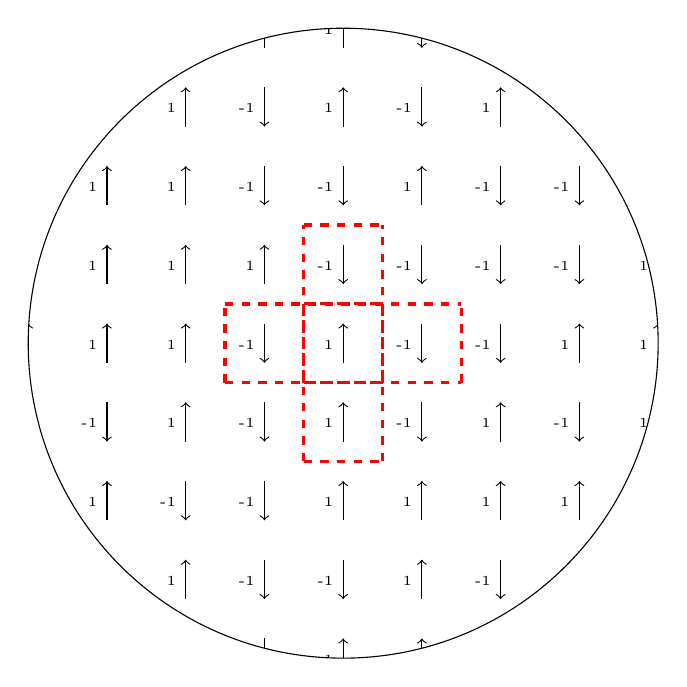
\begin{tikzpicture}
    \clip[draw] (-0.5,-0.5) circle (4cm);
    \draw (2.5,2.5) grid (3,3);
    \foreach \x in {-4,...,4} {
      \foreach \y in {-4,...,4} {
	\pgfmathsetmacro\dir{sign(rnd - 0.5)};
	\draw[->=latex, anchor=mid east] ( \x-0.5,\y-0.5)   (\x-0.5,\y-\dir/4 -0.5) -- ( \x-0.5,\y+\dir/4-0.5 )
	node[pos=0.5] 	{ \tiny \dir }  ;
	}
    };
    \draw[dashed,color=red,very thick] (-2,-1) grid (1,0) ;
    \draw[dashed,color=red,very thick] (-1,-2) grid (0,1) ;
  \end{tikzpicture}

\end{document}
